\section{Constructing the Pinhole Camera Model}

\subsection{Nomenclature}
\begin{figure}[H]
    \centering
    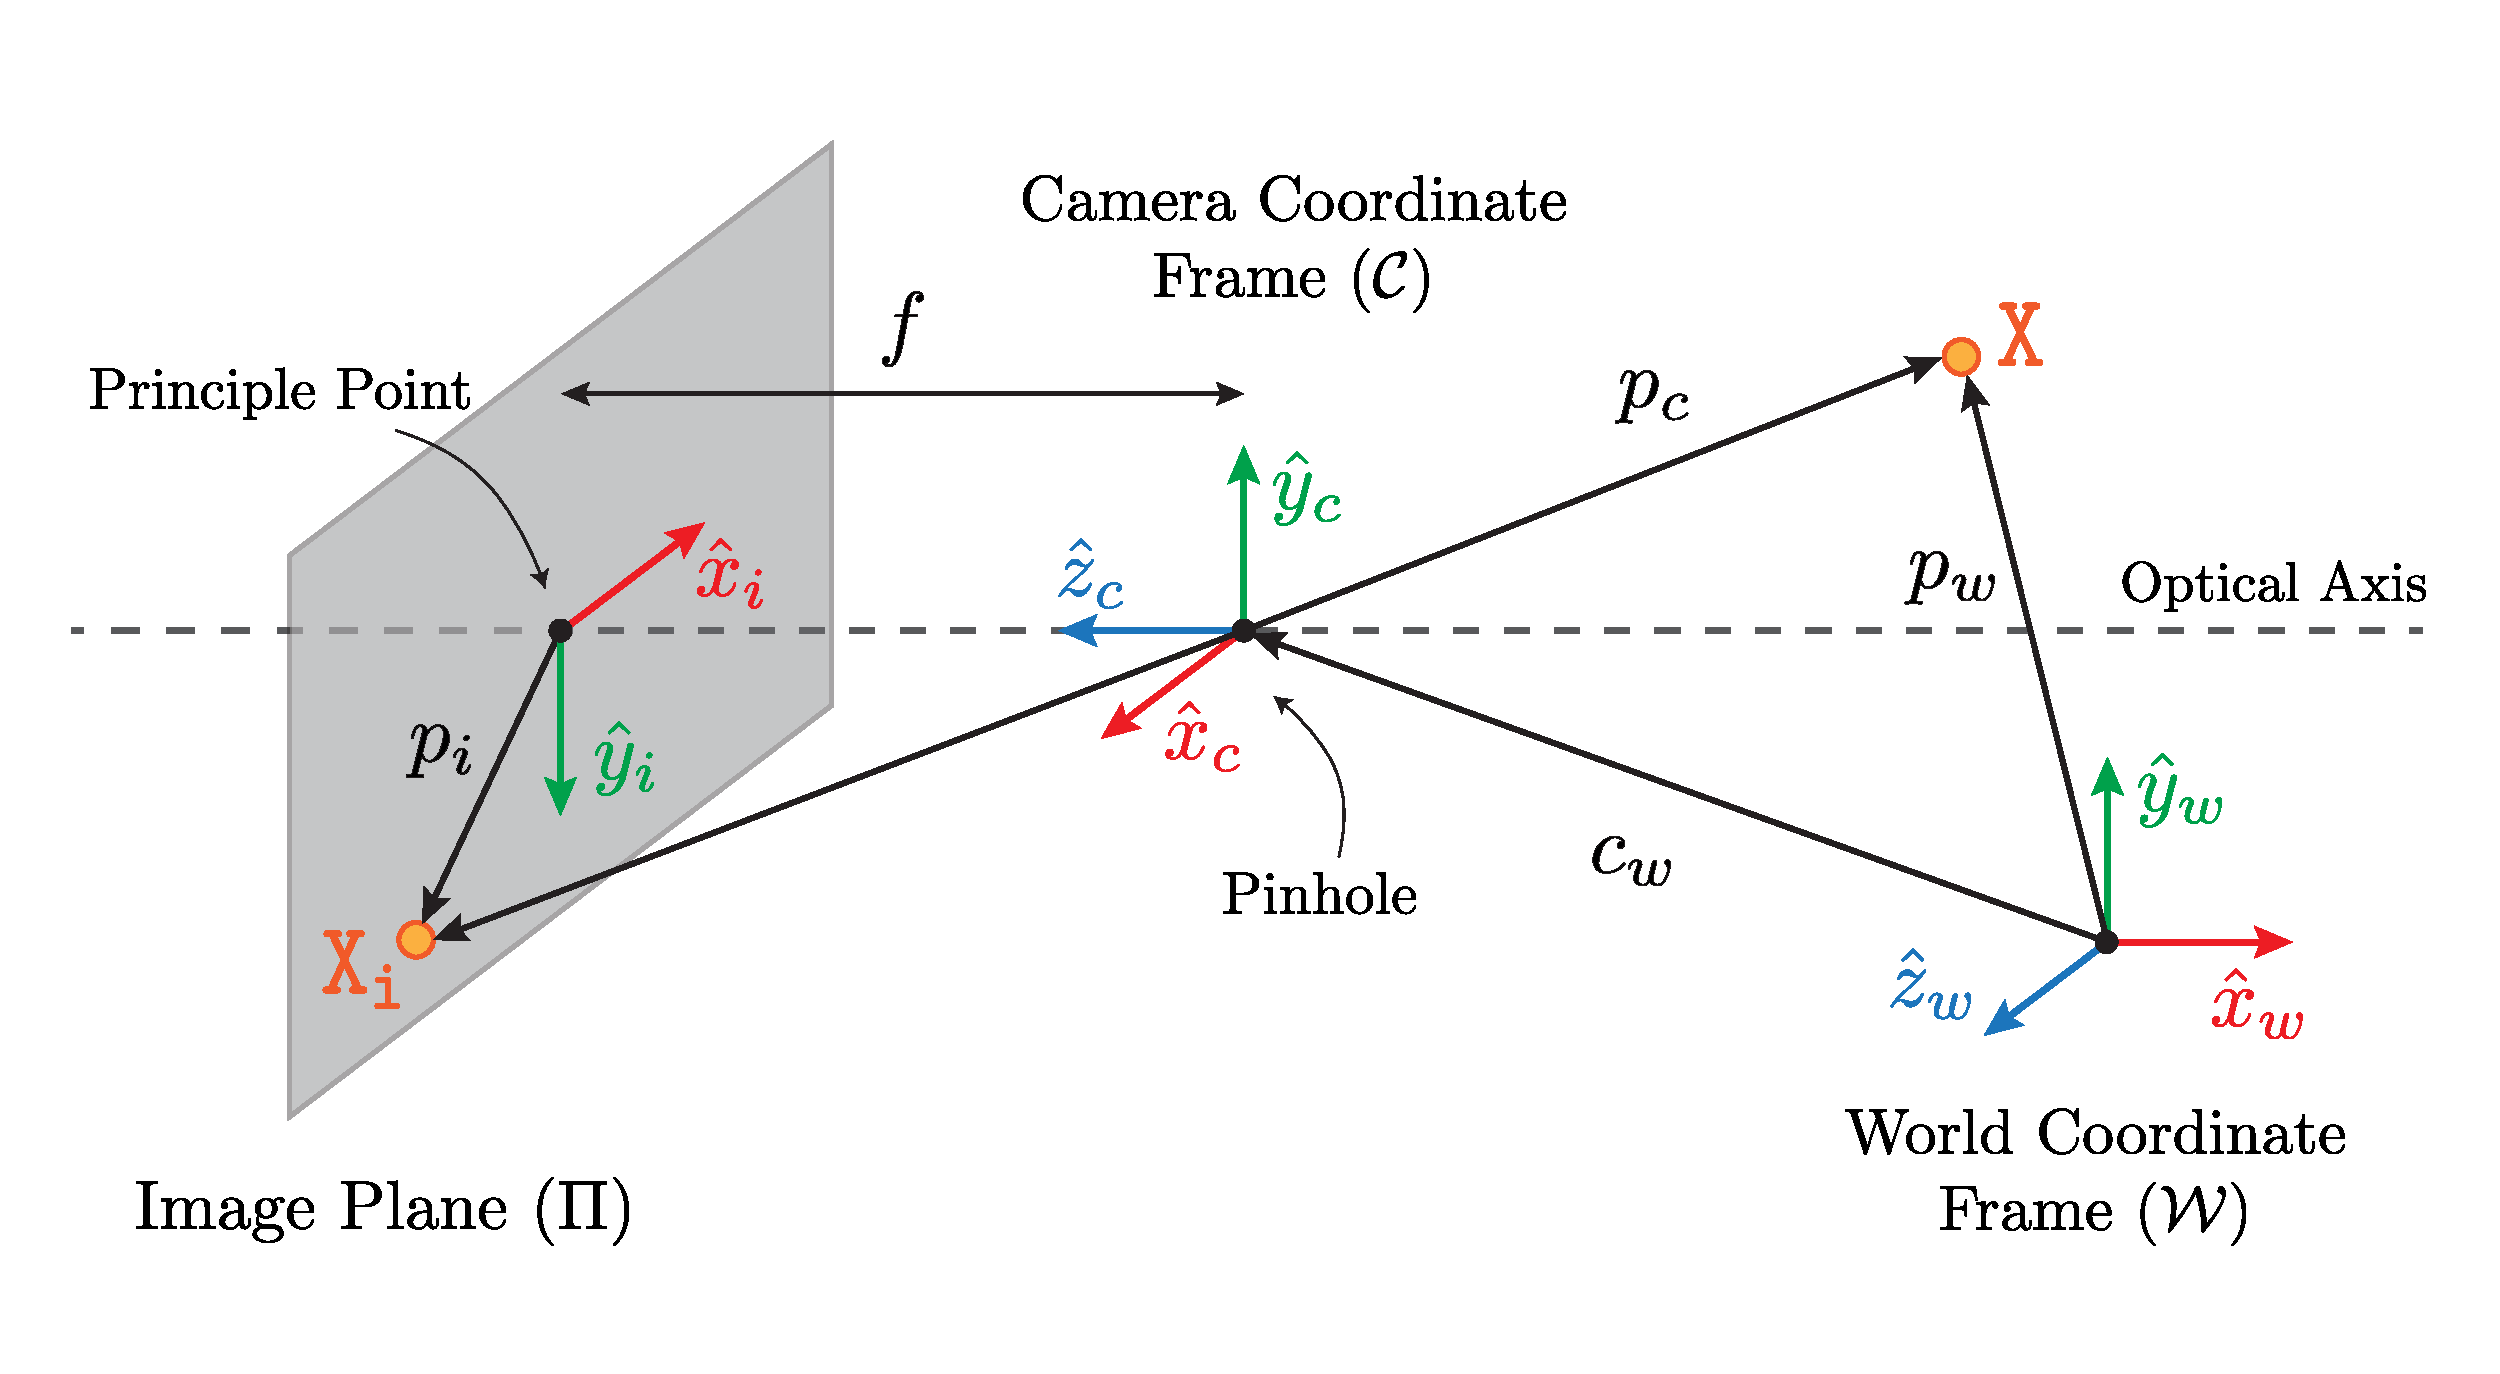
\includegraphics[width=0.9\textwidth]{figures/imaging_model}
    \caption{Pinhole camera model.}
\end{figure}

For our camera model, we will introduce 4 different coordinate systems:
\begin{itemize}[leftmargin=!, itemindent=-4ex]
    \item\textbf{The World Coordinate Frame $\boldsymbol{\mathcal{W}}$}. Points are denoted as $[x_w, y_w, z_w]^\T$
    \item\textbf{The Camera Coordinate Frame $\boldsymbol{\mathcal{C}}$}. Points are denoted as $[x_c, y_c, z_c]^\T$.
    \item\textbf{The Image Plane $\boldsymbol{\Pi}$}. Points are denoted as $[x_i, y_i]^\T$.
    \item\textbf{The Sensor Grid}. Points are denoted as $[u, v]^\T$.
\end{itemize}




\begin{figure}[H]
    \centering
    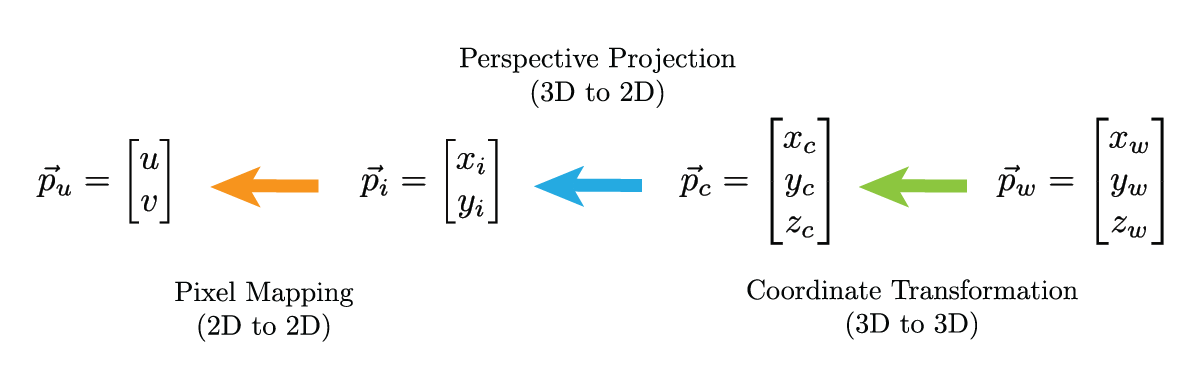
\includegraphics[width=0.9\textwidth]{figures/coord_conversions}
    \caption{Coordinate remappings.}
\end{figure}


\subsection{Intrinsic Parameters} \label{sec:intrinsics}

First, we will focus on the projection of points in the 3D space onto the image plane. The goal is to construct a calibration matrix, $K$, which relates the position of the point $P$ to its projection on the image plane. This can be expressed mathematically as follows:
\begin{equation} \label{eq:pi}
    \widetilde{p}_i =  K\widetilde{p}_c
\end{equation}
where $\vec{p}_i$ and $\vec{p}_c$ represents the position of $P$ in the image plane $\Pi$ and the camera frame $\mathcal{C}$ respectively.

\begin{figure}[H]
    \centering
    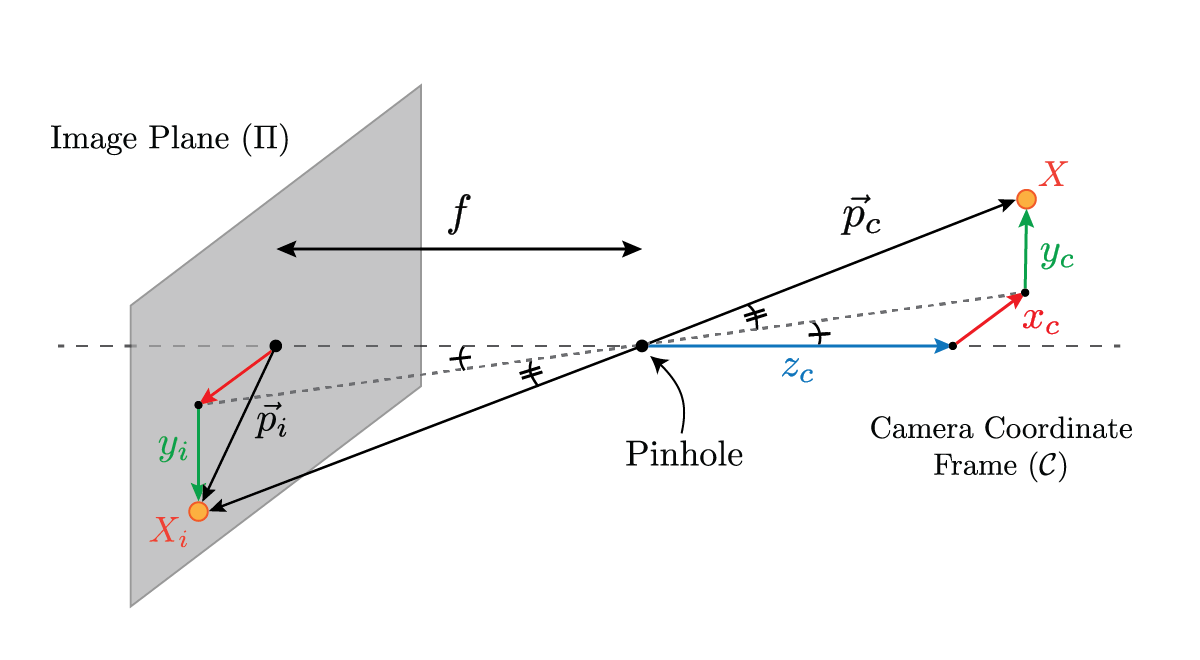
\includegraphics[width=0.9\textwidth]{figures/perspective_projection}
    \caption{Perspective projection of the point $P$ onto the image plane $\Pi$.}
\end{figure}

When a straight line is drawn from $P$ to its projection $P_i$ through the aperture, it intersects the optical axis. Deconstructing this intersection in the $x$ and $y$ direction, pairs of similar triangles are formed on the $x$ and $y$ plane. This is visualized in figure \ref{fig:similar_triangles}
\begin{figure}[H] \label{fig:similar_triangles}
    \centering
    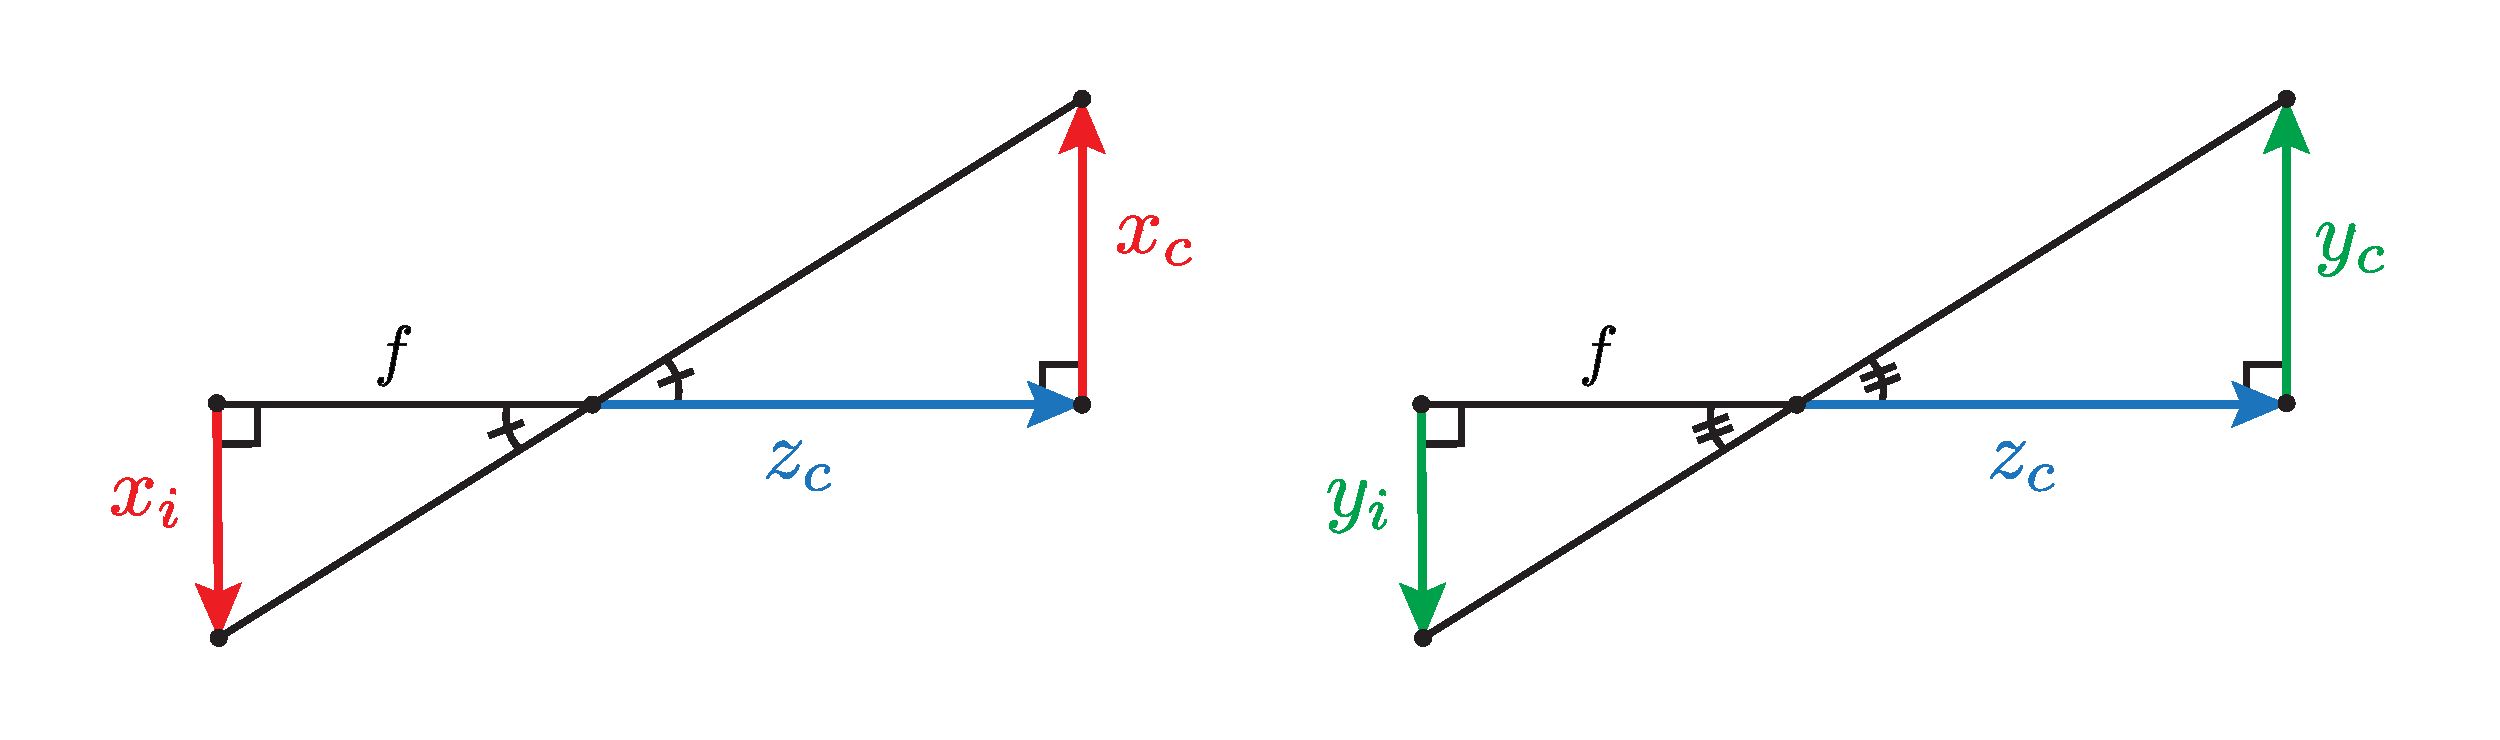
\includegraphics[width=\textwidth]{figures/similar_triangles}
    \caption{Similar triangles formed by perspective projection, which relate $x_i$ to $x_c$ and $y_i$ to $y_c$}
\end{figure}

\begin{subequations}
    \begin{gather}
        \frac{x_i}{f} = \frac{x_c}{z_c} \quad \Longrightarrow \quad x_i = f \frac{x_c}{z_c} \label{subeq:xi_result}\\
        \frac{y_i}{f} = \frac{y_c}{z_c} \quad \Longrightarrow \quad y_i = f \frac{y_c}{z_c} \label{subeq:yi_result}
    \end{gather}
\end{subequations}

We can then relate the coordinates of the projection, $(x_i, y_i)$, which are in real-world units, to its position $(u, v)$ in pixels.
\begin{figure}[H]
    \centering
    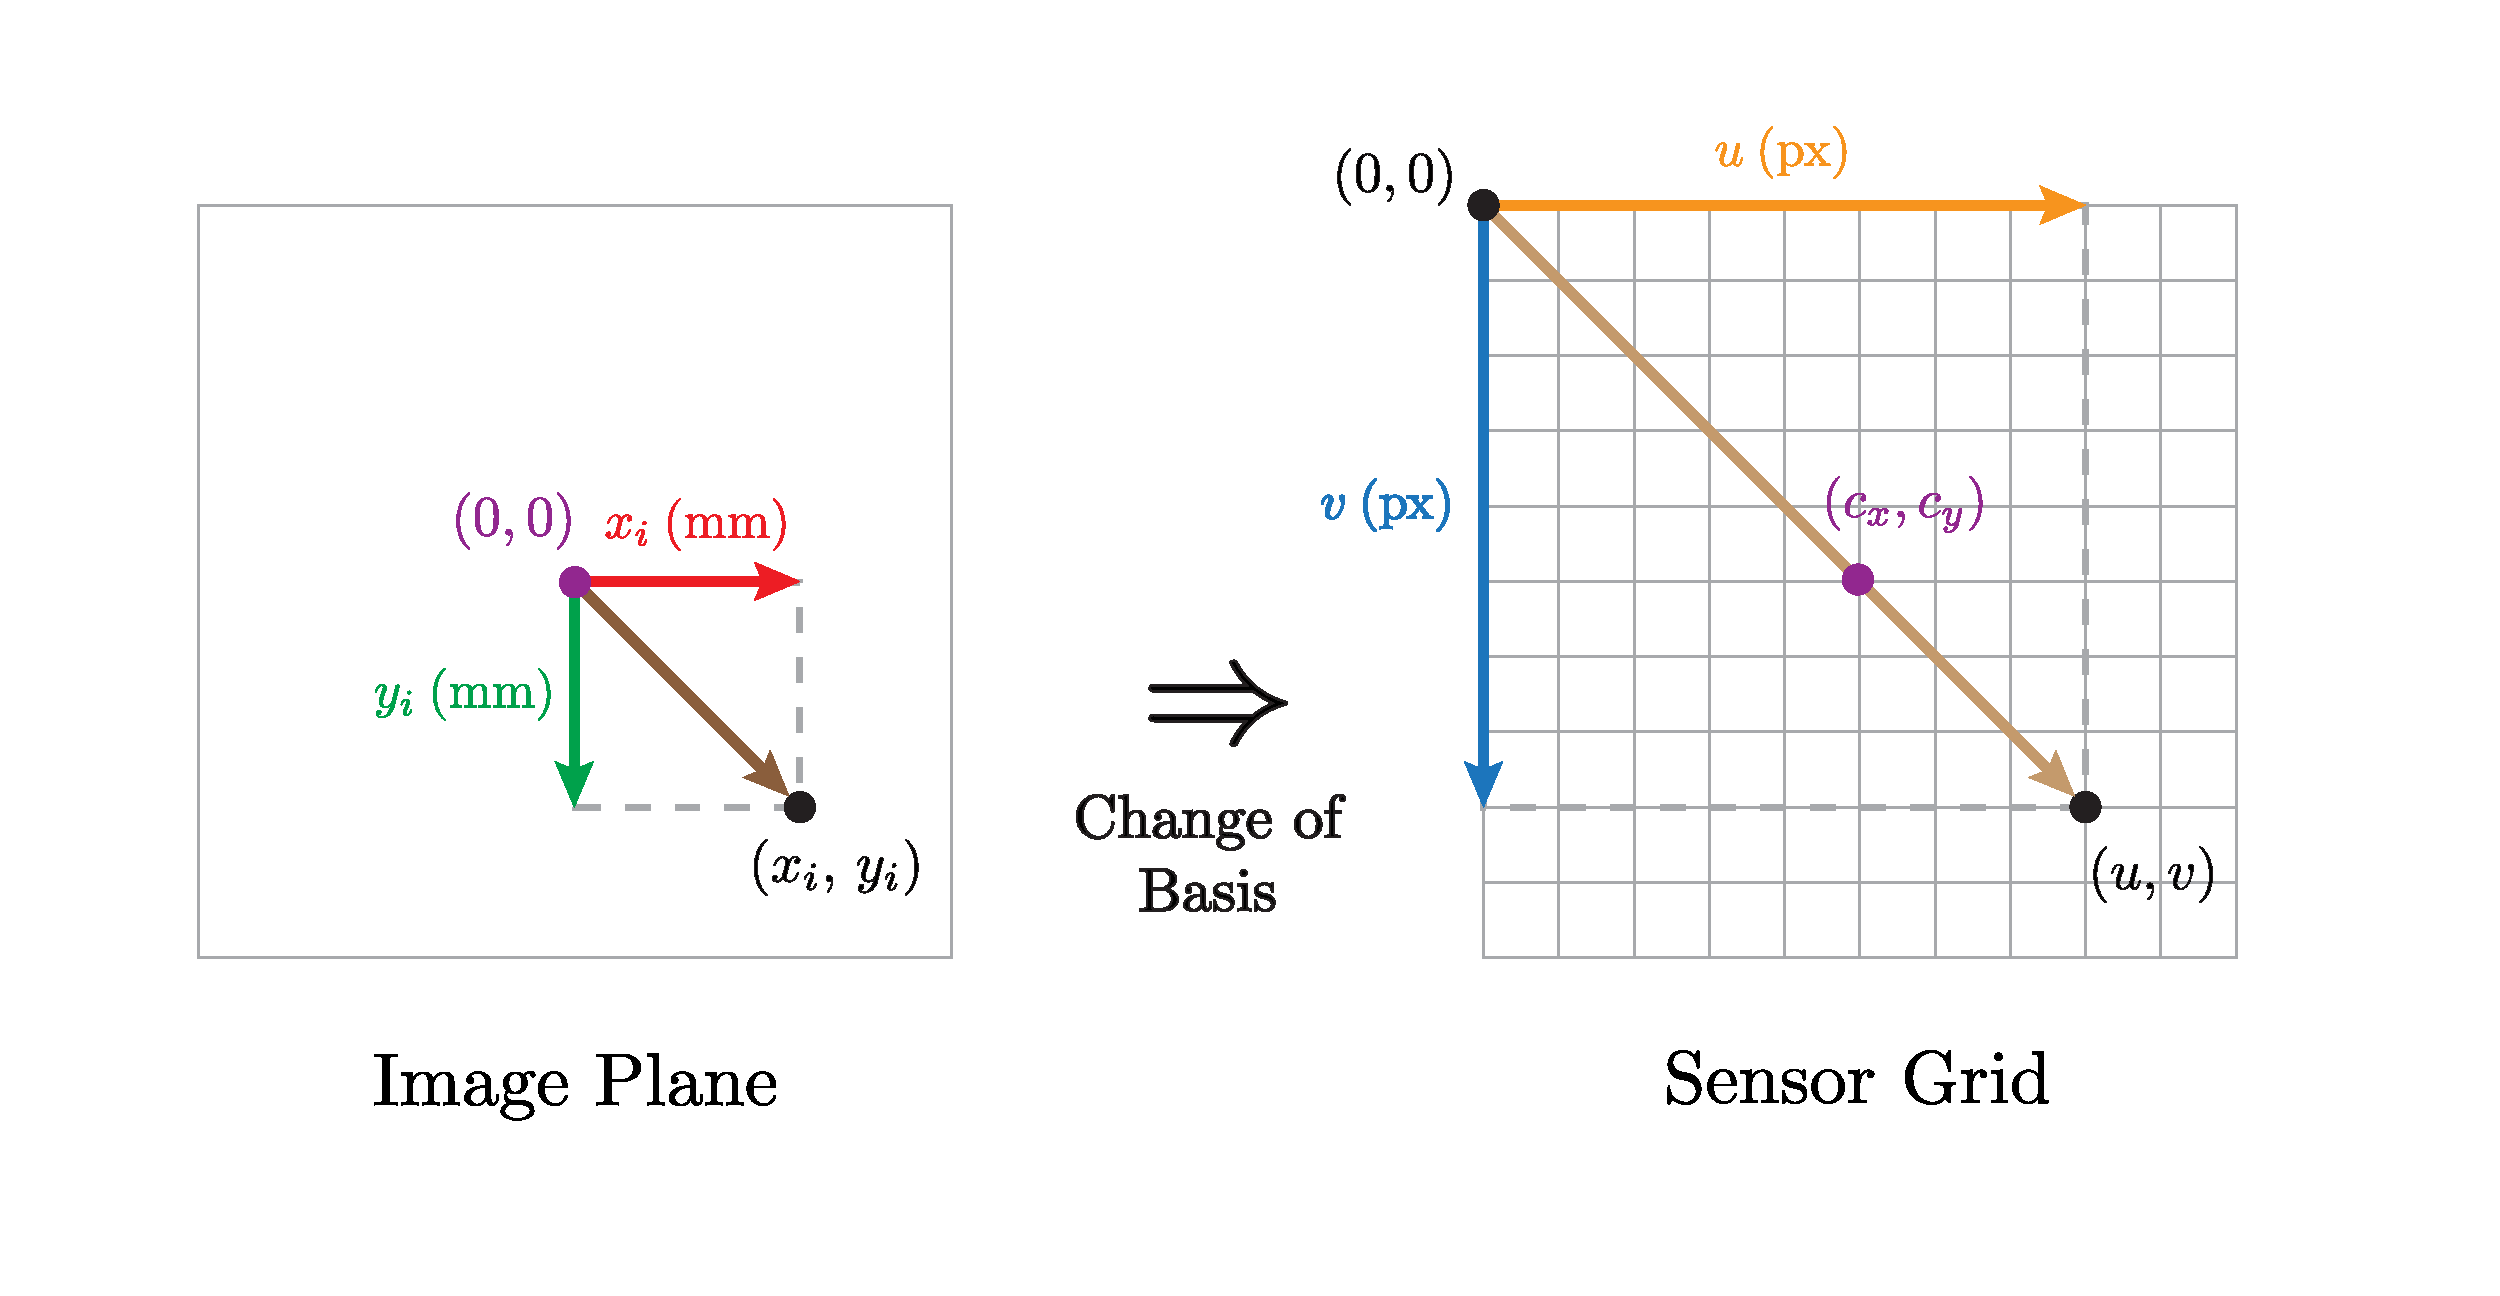
\includegraphics[width=\textwidth]{figures/sensor_grid}
    \caption{Conversion from image plane coordinates to sensor grid coordinates}
\end{figure}
Let $m_x$ and $m_y$ represent the pixel density of the image sensor in the $x$ and $y$ axes of the image sensor plane respectively.
\begin{align*}
    u = m_x x_i + c_x \\
    v = m_y y_i + c_y
\end{align*}
Replacing $x_i$ and $y_i$ for the result we obtained from \ref{subeq:xi_result} and \ref{subeq:yi_result}, we get:
\begin{align*}
    u = m_x f \frac{x_c}{z_c} + c_x \\
    v = m_y f \frac{y_c}{z_c} + c_y
\end{align*}
Since $m_x$, $m_y$, and $f$ are all unknowns, we can combine the products $m_x f$ and $m_y f$ to $f_x$ and $f_y$ respectively. Under this new scheme, we define $f_x$ and $f_y$ as the horizontal and vertical focal lengths of camera.
\begin{subequations}
    \begin{gather}
        u = f_x \frac{x_c}{z_c} + c_x \\
        v = f_y \frac{y_c}{z_c} + c_y
    \end{gather}
\end{subequations}

\begin{equation}
    \begin{bmatrix}
        u \\ v
    \end{bmatrix}
    \sim
    \begin{bmatrix}
        \widetilde{u} \\ \widetilde{v} \\ \widetilde{w}
    \end{bmatrix}
    \equiv
    \begin{bmatrix}
        z_c u \\ z_c v \\ z_c
    \end{bmatrix}
    =
    \begin{bmatrix}
        f_x x_c + z_c c_x \\ f_y y_c + z_c c_y \\ z_c
    \end{bmatrix}
    =
    \underbrace{
        \begin{bmatrix}
            f_x & 0   & c_x & 0 \\
            0   & f_y & c_y & 0 \\
            0   & 0   & 1   & 0
        \end{bmatrix}
    }_{\mathlarger{M_{int}}}
    \begin{bmatrix}
        x_c \\ y_c \\ z_c \\ 1
    \end{bmatrix}
\end{equation}


\begin{equation}
    K =
    \begin{bmatrix}
        f_x & 0   & c_x \\
        0   & f_y & c_y \\
        0   & 0   & 1
    \end{bmatrix}
\end{equation}

Note that $K$ that is an \emph{upper triangular matrix}. It is a special kind of square matrix with all of its non-zero entries above the main diagonal. This is an important property which we will exploit when extracting the intrinsic matrix from the projection matrix in section \ref{sec:projection}.

As such, we can express $M_{int}$ as $\left[\: K \:\vert\: 0 \:\right]$.

\begin{equation}
    M_{int} = \left[\: K \:\vert\: 0 \:\right]
\end{equation}

\subsection{Extrinsic Parameters} \label{sec:extrinsics}

Next, we will focus on finding the position 

Now, we would like to find the extrinsic matrix, $M_{ext}$, which relates the positional vector $\vec{p}_w$ of point $P$ in the world coordinate frame, to its positional vector $\vec{p}_c$ in the camera coordinate frame. Similar to what we did in section \ref{sec:intrinsics}, we can express this in homogenous coordinates as follows:
\begin{equation} \label{eq:pc}
    \widetilde{p}_c =  M_{ext}\,\widetilde{p}_w
\end{equation}

\begin{figure}[H]
    \centering
    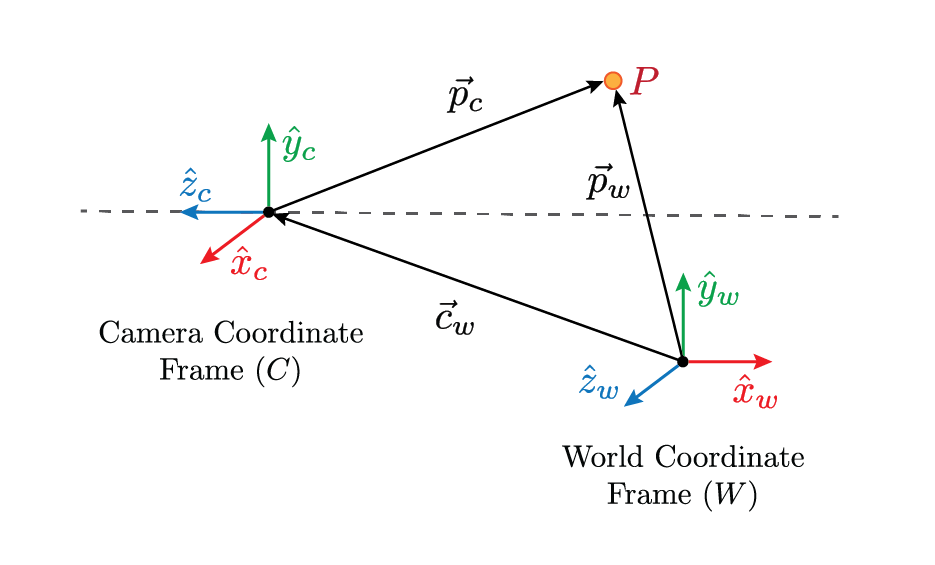
\includegraphics[width=0.9\textwidth]{figures/coord_transform}
    \caption{Coordinate transformation from the world coordinate frame to the camera frame.}
\end{figure}


For the extrinsic parameters of the camera, we have the position $\vec{c}_w$ of the camera in world coordinates and orientation $R$ of the camera. The orientation, $R$, is a 3x3 rotational matrix: 

\begin{equation}
    R = 
    \begin{bmatrix}
        r_{11} & r_{12} & r_{13} \\
        r_{21} & r_{22} & r_{23} \\
        r_{31} & r_{32} & r_{33}
    \end{bmatrix}
\end{equation}

\noindent where:
\begin{itemize}
    \item Row 1: Direction of $\hat{x}_c$ in world coordinate frame.
    \item Row 2: Direction of $\hat{y}_c$ in world coordinate frame.
    \item Row 3: Direction of $\hat{z}_c$ in world coordinate frame.
\end{itemize}

\noindent 

\begin{subequations}
    \begin{align}
        \vec{p}_c & = R(\vec{p}_w-\vec{c}_w) \\
                  & = R\vec{p}_w -R\vec{c}_w  
    \end{align}
\end{subequations}



\begin{gather}
    \vec{p}_c = R\vec{p}_w + \vec{t} \\
    \begin{bmatrix}
        x_c \\ y_c \\ z_c
    \end{bmatrix}
    =
    \underbrace{
        \begin{bmatrix}
            r_{11} & r_{12} & r_{13} \\
            r_{21} & r_{22} & r_{23} \\
            r_{31} & r_{32} & r_{33}
        \end{bmatrix}
    }_{\mathlarger{R}}
    \begin{bmatrix}
        x_w \\ y_w \\ z_w
    \end{bmatrix}
    +
    \underbrace{  
        \begin{bmatrix}
            t_x \\ t_y \\ t_z
        \end{bmatrix}
    }_{\mathlarger{\vec{t}}}
\end{gather}


\begin{equation}
    \begin{bmatrix}
        x_c \\ y_c \\ z_c \\ 1
    \end{bmatrix}
    =
    \underbrace{
        \begin{bmatrix}
            r_{11} & r_{12} & r_{13} & t_x \\
            r_{21} & r_{22} & r_{23} & t_y \\
            r_{31} & r_{32} & r_{33} & t_z \\
            0      & 0      & 0      & 1
        \end{bmatrix}
    }_{\mathlarger{M_{ext}}}
    \begin{bmatrix}
        x_w \\ y_w \\ z_w \\1
    \end{bmatrix}
\end{equation}

\begin{equation}
    M_{ext} = 
    \begin{bmatrix}
        R_{3 \times 3} & t_{3 \times 1} \\
        0_{1 \times 3} & 1
    \end{bmatrix} 
\end{equation}

\subsection{Putting It All Together}

When we combine the equations $\widetilde{p_c} = M_{ext}\,\widetilde{p}_w$ (eq. \ref{eq:pc}) and $\widetilde{p}_i = M_{int}\,\widetilde{p}_c$ (eq. \ref{eq:pi}), we obtain
\begin{equation} \label{eq:combined}
    \widetilde{p}_{i} = M_{int}\,M_{ext}\,\widetilde{p}_{w}
\end{equation}
To simplify our camera model, we can define a new matrix, $P \in \mathbb{R}^{3 \times 4}$, which is equal to the product $M_{int}\,M_{ext}$. Since $M_{ext}$ is a $4 \times 4$ matrix and $M_{int}$ is a $3 \times 4$ matrix, their matrix product produces a $3 \times 4$ matrix.
\begin{equation}  
    P=
    \begin{bmatrix}
        p_{11} & p_{12} & p_{13} & p_{14} \\
        p_{21} & p_{22} & p_{23} & p_{24} \\
        p_{31} & p_{32} & p_{33} & p_{34}
    \end{bmatrix}
    \equiv
    \underbrace{
        \begin{bmatrix}
            f_x & 0   & c_x  \\
            0   & f_y & c_y  \\
            0   & 0   & 1   
        \end{bmatrix}
    }_{\mathlarger{K}}
    \underbrace{
        \begin{bmatrix}
            r_{11} & r_{12} & r_{13} & t_x \\
            r_{21} & r_{22} & r_{23} & t_y \\
            r_{31} & r_{32} & r_{33} & t_z \\
        \end{bmatrix}
    }_{\mathlarger{\left[\,R\,\vert\,\vec{t}\:\right]}}
\end{equation}

Replacing $P$ for $M_{int}\,M_{ext}$ in equation \ref{eq:combined}, we obtain
\begin{equation} \label{eq:project}
    \widetilde{p}_{i} = P\,\widetilde{p}_{w}
\end{equation}
The implications of this equation is very important, as it means that we can project the $n$th point $\left[ x_w^{(n)}, y_w^{(n)}, z_w^{(n)} \right]^\T$ in the world coordinate frame $\mathcal{W}$ to its pixel coordinates $\left[ u_n, v_n \right]^\T$ on the image plane $\Pi$ simply by using the projection matrix. But now, we need to figure out a way to solve for the project matrix. 

Given that we have equation \ref{eq:project} which relates 



When expressing the pixel coordinate in homogenous coordinates, equation \ref{eq:project} becomes
\begin{equation}
    \begin{bmatrix}
        u_n \\ v_n
    \end{bmatrix}
    \sim
    \begin{bmatrix}
        \widetilde{u}_n \\ \widetilde{v}_n \\ \widetilde{w}_n
    \end{bmatrix}
    =
    \begin{bmatrix}
        p_{11} & p_{12} & p_{13} & p_{14} \\
        p_{21} & p_{22} & p_{23} & p_{24} \\
        p_{31} & p_{32} & p_{33} & p_{34}
    \end{bmatrix}
    \begin{bmatrix}
        x_w^{(n)} \\ y_w^{(n)} \\ z_w^{(n)} \\ 1
    \end{bmatrix}
\end{equation}
